\documentclass{eceasst}
% This is an empty ECEASST article that can be used as a template
% by authors.
% Just uncomment the appropriate frontmatter commands and provide
% the parameters.

% Required packages
% =================
% Your \usepackage commands go here.

% Volume frontmatter
% ==================
% Volume frontmatter for AVoCS 2015
% =====================================
\volume{XXX}{2015} % Volume number and year
\volumetitle{% Title of the volume (optional)
Proceedings of the\\
15th International Workshop on\\
Automated Verification of Critical Systems
(AVoCS 2015)}
\volumeshort{% Short title of the volume (optional)
Proc.\ AVoCS 2015}
\guesteds{% Multiple guest editors
Gudmund Grov, Andrew Ireland}


% Article frontmatter
% ===================
\title{Scaling Automated Theory Exploration} % Title of the article
%\short{} % Short title of the article (optional)
\author{Chris Warburton\sponsor{}} % Authors and references to addresses
\institute{ % Institutes with labels
\email{cmwarburton@dundee.ac.uk}\\
School of Computing\\
University of Dundee}
\abstract{
We investigate the \textbf{theory exploration} (TE)
paradigm for computer-assisted Mathematics and identify limitations and
improvements for current approaches. Unlike the theorem-proving paradigm,
which requires user-provided conjectures, TE performs an open-ended
search for theorems satisfying given criteria. We see promise in TE for
identifying new abstractions and connections in libraries of software
and proofs, but realising this potential requires more scalable
algorithms than presently used.} % Abstract of the article
%\keywords{} % Keywords for the article

\begin{document}
\maketitle

% Main part of your article
% =========================
\section{Introduction}

The \emph{theory exploration} (TE) paradigm provides software support
for traditional Mathematical workflows; namely, deriving ``interesting''
consequences from formal definitions \cite{RISC1482}. Early
implementations like \textsc{Theorema} \cite{buchberger2000theory} provided
interactive environments, similar to computer algebra systems like
\textsc{Mathematica} (in which \textsc{Theorema} is implemented) or
interactive theorem provers. Subsequent systems have investigated
\emph{automated} theory exploration, for tasks such as lemma discovery
\cite{Hipster}.

By removing user interaction, automated TE systems require an algorithm
for deciding whether to inform the user of a particular theorem or not; we refer
to this search criterion as the theorem being ``interesting''. In existing
systems, this criterion is intimately connected to the
search algorithm; such coupling improves efficiency, even for brute-force
search, but makes it difficult to try alternative measures.

As an example, \textsc{IsaCoSy} \cite{johansson2009isacosy} discovers
equations, which are defined as ``interesting'' if they cannot be simplified
using previously discovered equations. The intuition for such criteria is to
avoid special cases of known theorems, such as $0 + 0 = 0$, $0 + 1 = 1$,
etc. when we already know $\forall x. 0 + x = x$. Whilst elegantly implemented
as a term rewriting system, to work effectively this requires general forms to
be found \emph{before} special cases.

In the following, we give an overview of the state of the art in automated
theory exploration (\autoref{haskell}). We identify potential improvements to
these systems (\autoref{improve}) and present our initial implementation
attempts in the form of the \textsc{ML4HS} system (\autoref{ml4hs}).

\section{Theory Exploration in Haskell}\label{haskell}

Automated theory exploration has been applied to libraries in Isabelle
and Haskell, although we focus on the latter as its implementations are
the most mature (demonstrated by the fact that \textsc{Hipster} explores
Isabelle by first translating it to Haskell). Haskell is interesting to target,
since its use of pure functions and algebraic datatypes causes many programs to
follow algebraic laws. However, since Haskell's type system cannot easily
encode such laws, less effort is given to finding and stating them; compared to
a theorem proving setting like Isabelle.

Due to Haskell's relative popularity, there are also large code repositories
such as \textsc{Hackage} available to explore. This gives several potential
benefits: in the short term, applying TE to such repositories may assist
existing library authors and users in comprehending and maintaining their code
\cite{QuickSpec}; more notably, TE could be used to data mine new abstractions,
such as typeclasses, with relevance to real-world applications.

Currently, the most powerful TE system for Haskell is \textsc{HipSpec}.
This uses the earlier \textsc{QuickSpec} system to search through
\emph{expressions} (combinations of the Haskell terms given by the theory),
rather than searching through the space of equations or proofs directly.
Expressions are grouped into equivalence classes, such that the
\textsc{QuickCheck} counterexample finder cannot distinguish between the
elements; equations relating the members of these classes are then conjectured,
and sent to existing automated theorem provers to try and prove
\cite{rosen2012proving}. This approach works well as a lemma generation system,
making \textsc{HipSpec} a capable inductive theorem prover as well as a theory
exploration system \cite{claessen2013automating}.

\section{Identifying Improvements}\label{improve}

Given this state of the art, we identify the following as potential
areas for investigation:

\begin{itemize}
\item
  More scalable alternatives to brute-force enumeration. This is a well-studied
  area of Artificial Intelligence and Machine Learning. In particular, there is
  potential in applying heuristic algorithms like those surveyed in
  \cite{blum2011hybrid}.
\item
  Using alternative ``interestingness'' criteria, like those surveyed in
  \cite{geng2006interestingness}. In particular, we envision two problems with
  large-scale exploration which may require more sophisticated criteria:

  \begin{itemize}
  \item
    As the number of irreducible equations grows, it may be desirable to
    impose extra conditions of a more subjective nature; e.g. to distinguish
    useful relationships from incidental coincidences.
  \item
    Surprising, insightful equations may be discarded by current systems, if
    they are actually reducible in some complex, non-obvious way. A more
    subjective interestingness measure could be used to veto such
    rejections.
  \end{itemize}
\item
  Data mining previous results; for example, using generalisation methods like
  anti-unification \cite{bulychev2010anti}. This would make more efficient use
  of data, and also remove the requirement that general forms be enumerated
  early.
\item
  Divide and conquer approaches. Rather than try all type-safe combinations of
  the given expressions, it may be discernable a priori that some combinations
  are not worth considering (either because they are never related, or because
  their relations are never interesting). In other words, automating the theory
  selection process currently performed by the user.
\end{itemize}

We consider all of these worth investigating, although in this paper we
focus on the last item.

\section{The \textsc{ML4HS} Framework}\label{ml4hs}

\begin{figure}
  \centering
  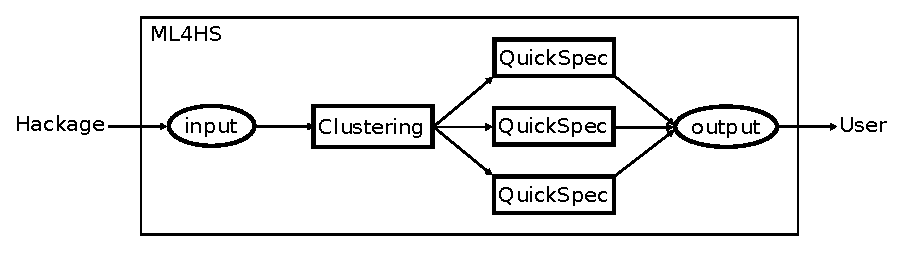
\includegraphics[]{ml4hs}
  \caption{An overview of the \textsc{ML4HS} system}
  \label{ml4hsdia}
\end{figure}

We are implementing a system called \textsc{ML4HS} to investigate scalable
automated theory exploration for Haskell. The current form of \textsc{ML4HS} is
a pre-processor for \textsc{QuickSpec} which attempts to make exploration of
large theories more tractable by splitting them into a collection of smaller
theories: the divide and conquer approach mentioned above. This is
similar to reducing the search space in automated theorem proving via premise
selection \cite{kuhlwein2012overview}. The basic idea of \textsc{ML4HS} is shown
in \autoref{ml4hsdia}: theories, in the form of Haskell packages, are split up
and sent to concurrent instances of QuickSpec, and the results collated.

When selecting the components of each sub-theory, we want to keep together those
expressions which combine to form interesting theorems, and separate those which
combine in uninteresting ways. Our hypothesis is that similarity-based
clustering of expressions, as found in \textsc{ML4PG}
\cite{journals/corr/abs-1302-6421}, is an effective method for performing this
division. Future experiments will test this by measuring throughput rates of
\textsc{ML4HS} compared to \textsc{QuickSpec} and \textsc{HipSpec}.

% Acknowledgements for colleagues, referees, ...
% ==============================================
\begin{acknowledge}
Thank you to the \textsc{HipSpec} team at Chalmers University (Moa Johansson,
Koen Claessen, Nick Smallbone, Dan Ros{\'e}n and Irene Lobo Valbuena) for useful
discussions of these ideas.
\end{acknowledge}

% Bibliography with BibTeX
% ========================
\bibliographystyle{eceasst}
\bibliography{../Bibtex}

\end{document}
